\section{广域网络路由异常}

\subsection{路由协议的固有缺陷}

广域网络的路由事实上是非常脆弱而易受攻击的。实际上,BGP 最初被提出以来,没有任何被协议所直接包括的安全机制\citing{mitseva2018state},路由的稳定可靠完全是基于网络运营商之间的信任和恰当的设置,也即假定系统永远不会出现随机故障或安全问题,路由器之间不会发送错误的数据。这引入了一个明显的漏洞:如果路由协议的其中某个参与方出于恶意,试图通过BGP协议影响其它自治系统乃至全球的路由表,其它的自治系统没有任何通用的手段来阻止它的发生。

在 1998 年,RFC2385 对 BGP 引入了密码保护机制\citing{heffernan1998protection},解决了通过二层链路劫持 BGP 会话的可能性,但它使用易受攻击的 MD5 加密,至今尚未更改。1999 年,RFC2439 对 BGP 引入了路由震荡抑制(Route Damping)\citing{villamizar1998bgp}机制,缓解了 BGP 的路由震荡问题。然而,在标准提出的几十年来,广域网络上的路由异常问题从来没有得到根除,究其原因有二:

其中一个原因是针对底层协议和标准的修改难以被普遍采纳。一项报告指出,互联网运营商的核心设备的更新周期长达 10-15 年,并拥有相当大的方差\citing{mahimkar2010detecting},这意味着在新的标准提出后,大部分设备都很难短时间内进行引入\citing{mitseva2018state},或是为了与其它互连的运营商兼容的原因关闭这些增强安全性的功能。

另一个重要原因是,这些手段事实上并未解决来自恶意的路由协议参与者和不遵循规范的配置者的安全威胁\citing{sermpezis2018survey}。基于信任的广域网架构仍然坚持默认所有路由参与者不会存在恶意破坏的可能性,这是维持互联网分布式的基础。

因而,由此产生的安全性问题,包括路由异常问题,便从标准性问题转变为了无法避免的问题,它的潜在安全威胁使得对路由系统的安全性的建模研究更具意义。

\subsection{广域网络的潜在安全威胁}

% \subsubsection{路由震荡}

% 路由震荡是指由于物理故障、系统错误、人为因素等原因,所造成的路由表的频繁变化。相互连接的分布式网络会因此不断向相邻自治系统宣告和撤回路由,导致其他节点频繁重新计算路由。这会对整个网络造成严重的算力和链路负担,轻则网络延迟升高、不稳定,重则导致拒绝服务攻击(Denial of Service,DOS),并造成大规模的网络服务瘫痪。

% 这样的问题可以通过修改外部网关协议的行为,来防止系统资源的枯竭,例如在 BGP 协议中启用路由震荡抑制功能,临时关闭反复路由更新的邻接系统的 BGP 会话,或是限制对应协议的更新频率。

% \subsubsection{路由劫持}

路由劫持是广域网中最常见的安全威胁。当一个自治系统因为配置错误或恶意行为的情况下,它会宣告并不应由它宣告的路由条目,如果它的邻接系统没有部署 RPKI 机制或是没有强制启用路由的过滤机制,这些错误的路由条目就会通过 BGP 会话传播到它的邻接系统,并进而被发送至整个广域网内所有可达的边界路由器中,这时候路由劫持事件即被触发,由于 BGP 路由协议的规则影响,目的地涉及到被劫持的 IP 地址块的网络流量有可能会被路由至发起劫持的自治系统\citing{mitseva2018state}。而现代互联网的系统反应时间非常迅速,根据一项调查显示\citing{sermpezis2018survey},被劫持的路由条目能够在 10 秒时间内抵达全球 90\% 以上的互联网系统。

并非所有的 BGP 劫持都能够成功造成安全危害,事实上,对网络的拓扑结构造成更大影响的 BGP 劫持通常能有能力影响更多或具有更大客户锥形的自治系统,这通常有两种方式:

\begin{enumerate}
    \item 发起劫持的自治系统宣告前缀长度更长的路由。网络系统的路由层次性决定了路由器在接收到更准确的IP地址块的路由信息的时候,会直接采用并完全弃用任何路径选择算法。
    \item 提供更为直接的自治系统路径,利用广域网路由选择算法的特点,构造出比正常路由更短的自治系统路径,这将使得路由器认为该路由在逻辑上更优。
\end{enumerate}

% 大型网络或网络群的运营商(其中很多是ISP)会明目张胆地进行这种恶意活动,这似乎令人惊讶。但考虑到据统计,现在全球有超过8万个自治系统,有些自治系统不值得信任也就不足为奇。此外,BGP劫持并不总是那么明显或容易被发现。坏人可能会把他们的活动伪装在其他自治系统的后面,或者宣布一些不可能被注意到的未使用的IP前缀块,以便不被发现。

图 \ref{bgp-hijack} 显示出了一种典型的基于更长前缀的路由劫持,AS3 通过向广域网宣告 1.14.5.0/24 这一更长的路由前缀,劫持了本应属于 AS1 的 1.14.0.0/16 的路由,并将访问 1.14.5.14 IP 的流量引导向攻击者的设备,整个流程中 AS1 及其 AS2 没有执行任何错误操作,同范围的其他 IP 也能通过一种称为流量穿透的方法返回正常目的地,从而实现隐蔽的攻击手段。

一些网络运营商可能因为配置失误,将内部或错误的路由发送至自治系统外,造成BGP劫持,这样的情况常常被称为路由泄露,据调查,此类事件相比于恶性的劫持事故而言往往更加常见\citing{vervier2015mind}。根据一项研究显示,并不是所有的 BGP 劫持事件都能够被注意到并及时采取措施\citing{schlamp2016heap},攻击者可以选择不常使用的地址块,或是未被注册的地址块进行劫持。以上原因都导致了路由异常的检测实质上难以判断是否是恶意攻击行为。

\begin{figure}[h]
    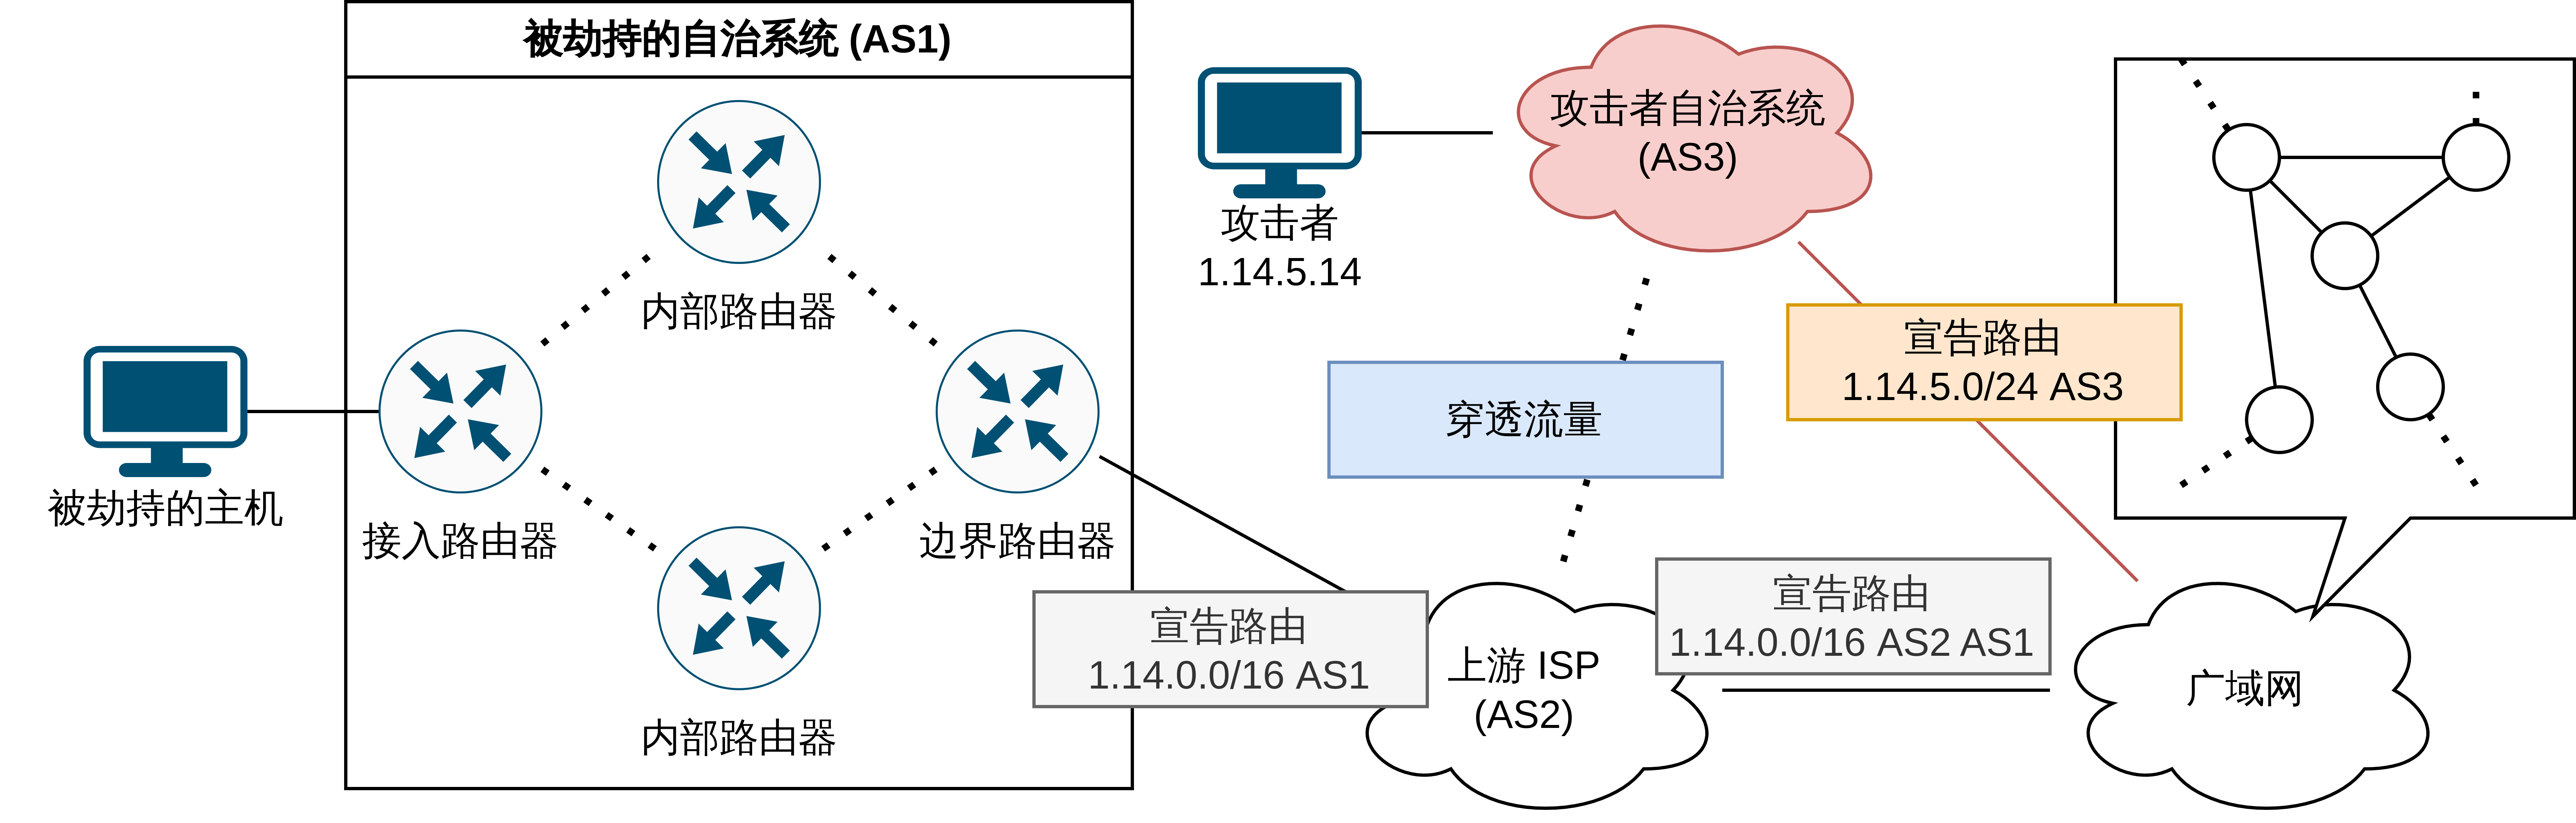
\includegraphics[width=\linewidth]{chapter/c2_images/c2_hijack.png}
    \caption{BGP劫持示意}
    \label{bgp-hijack}
\end{figure}

\subsection{路由异常的定义}

路由异常,被定义为一种表现出异常特征的路由更新条目,它通常携带有异于其它正常路由拓扑的自治系统路径,并有可能在其它属性上呈现出不同的特点\citing{al2016bgp}。它一般包括两类状况,一种是 BGP 劫持,这类事件通常是有害的;而另一类是新路由的增加,由于分布式网络的系统之间常常建立和断开连接,这一类异常状况既可以是突发事件,也可以是可预测的人为因素,它们并不会产生实质性危害。

由于现有数据集中基于图网络的有标记路由异常事实上并不多见,此类问题一般被认为是一种无监督学习问题。

\subsection{问题的图网络表述}

% 使用基于图网络的数学公式描述问题。
下面通过图网络的数学语言描述本研究所定义的广域网络异常检测:

对于一条路由 $R_i$,它包含三种属性,即对应的 IP 前缀 C,AS 路径 P,社区信息 C,即 $R_i = \{ O, P, C \}$,它们共同组成全球路由表 $R_T = \{ R_i \}$。
% 全球路由表 {R_i} , R_i = {O(前缀), P(路径), C(社区)}

前缀 C 是一个标识符;AS 路径 P 可理解为一个不定长的有序列表 $P = \{A_1,A_2..A_N\}$,其中,路由的源自治系统指宣布该路由的自治系统,对应列表中的最后一个元素 $A_N$;社区信息 C 是一个标签集合 $C = \{C_1,C_2...C_N\}$。

% last(P) = origin

定义图生成算法 $f_g$ 为从路由表数据构造图网络数据集的方法,具体来说,$f_g(R_T)=G<V,E>$,其中节点集 V 是路由表 ${R_i}$ 中所有路由路径上的自治系统号码,即 $V = \forall(A_i \in P \in R_i)$,该算法通过 $R_i$ 特征生成一个有向或无向图 $G<V,E>$,它的边集 E 将由算法 $f_g$ 决定。
% 图生成算法 f_g({R_i})=G<V,E> V=all(P)

定义图嵌入算法 $f_e$ 为从图网络数据 $G<V,E>$ 中提取嵌入数据的方法,它对于每一个图元素输出一个 k 维向量嵌入,即 $e = f_e(G<V,E>) = \{ e_i \}$,而图元素可以是图上的所有节点,也可以是边集或是路径集,即 $N = len(V/E/R)$。
% 嵌入算法 e = f_e(G<V,E>)={e_i} N=num(V/E/R)

最后定义异常分数 $f_a$ 是由新的路由和原有的图数据及其嵌入作为输入,输出对更新路由的异常分数以便于最终进行异常检测,即 $f_a(R_n,G<V,E>,e) \in (0,1]$。
% 定义异常分数 f_a(R_n,G<V,E>,e)

广域网络的路由异常检测问题的本质即包含了以下的部分:

\begin{enumerate}
    \item 设计图生成算法 $f_g$,将原网路数据集转换为图数据集。
    \item 设计高效的嵌入算法 $f_e$,将图数据集转换为图元素的嵌入。
    \item 定义异常检测分数 $f_a$,用以检测新的测试样本。
\end{enumerate}
